\documentclass[11pt]{article}

\usepackage[margin=1in]{geometry}
\usepackage[T1]{fontenc}
\usepackage[utf8]{inputenc}
\usepackage{lmodern}
\usepackage{indentfirst}
\usepackage{microtype}
\usepackage{amsmath, amssymb}
\usepackage{booktabs}
\usepackage{graphicx}
\usepackage{array}
\usepackage{longtable}
\usepackage{multirow}
\usepackage{enumitem}
\usepackage{xcolor}
\usepackage{hyperref}
\usepackage[numbers,sort&compress]{natbib}

\hypersetup{
  colorlinks=true,
  linkcolor=blue!60!black,
  citecolor=blue!60!black,
  urlcolor=blue!60!black,
  pdftitle={What Determines Long-Context Ability in LLMs?},
  pdfauthor={}
}

\title{\textbf{What Determines Long-Context Ability in LLMs?}\\
\large \textbf{A Survey with Experimental Analysis}}
\author{Sihua Zhang, Minghao Xi}
\date{\today}

\begin{document}
\maketitle

\begin{abstract}
Long-context ability has become central to modern large language models (LLMs), yet the field still lacks a stable answer to a deceptively simple question: what does it mean for a model to use long context well? Larger context windows alone are insufficient. A model may accept 128K or even million-token inputs while degrading on retrieval from the middle of a document, on multi-hop aggregation across distant spans, or under realistic serving constraints. This report surveys long-context LLMs through a unified lens that separates five factors: nominal context length, effective retrieval length, long-range reasoning ability, inference-time extension effectiveness, and system serving efficiency. We review architectural routes for long-sequence modeling, context extension methods, retrieval and memory augmentation, and system techniques including IO-aware attention and KV-cache management. We further map the evaluation landscape from Needle-in-a-Haystack tests to RULER, LongBench, and LongBench v2. On the empirical side, we conduct a cross-architecture study on RULER NIAH retrieval, RULER reasoning, and LongBench tasks using Llama-3.1-8B-Instruct and Falcon3-Mamba-7B-Instruct, together with a system performance comparison across HuggingFace and vLLM backends. The results show that long-context failure does not emerge as a smooth curve but as task-dependent breakdown in key-value binding, position robustness, reasoning stability, and system feasibility. Our main claim is that long-context ability is a joint outcome of model architecture, task structure, inference policy, and system implementation.
\end{abstract}

\section{Introduction}
Large language models are deployed in settings that are inherently long-context: document QA, multi-document synthesis, repository-scale code understanding, long-horizon agent memory, and structured analysis over extended logs. These scenarios have driven rapid growth in nominal context windows---from a few thousand tokens to 32K, 128K, and beyond. Yet the field has accumulated evidence that accepting longer inputs is not the same as using them effectively \citep{liu2024lost, hsieh2024ruler, bai2024longbench, kuratov2024babilong, bai2025longbenchv2}.

This mismatch appears in several ways. Position-sensitive evaluations show that models often underuse information placed in the middle of long prompts \citep{liu2024lost}. Synthetic benchmarks beyond single-needle retrieval reveal a gap between claimed and effective context size \citep{hsieh2024ruler}. Realistic multi-task evaluations suggest that deeper reasoning, rather than nominal window size, is now the main long-context bottleneck \citep{bai2025longbenchv2}. Meanwhile, systems work shows that deployment is constrained by prefill latency, KV-cache growth, and batching efficiency even when the model is theoretically capable of longer inputs \citep{dao2022flashattention, kwon2023pagedattention, zheng2024sglang}.

This report is organized around a single question: \emph{what determines long-context ability in LLMs?} We decompose it into five dimensions:
\begin{enumerate}[leftmargin=1.5em]
  \item \textbf{Nominal context length}: how many tokens the model and serving stack claim to support.
  \item \textbf{Effective retrieval length}: how far relevant information can be reliably retrieved.
  \item \textbf{Long-range reasoning ability}: whether the model can aggregate, compare, and reason over distant evidence.
  \item \textbf{Inference-time extension effectiveness}: how much usable context can be recovered without retraining.
  \item \textbf{System serving efficiency}: whether the model can run with acceptable latency, memory, and throughput.
\end{enumerate}

Section~\ref{sec:framework} formalizes this framework. Sections~\ref{sec:modeling}--\ref{sec:systems} survey modeling, extension, retrieval, and systems techniques. Section~\ref{sec:evaluation} reviews benchmarks and what they measure. Section~\ref{sec:experiments} presents our experimental study across retrieval, reasoning, and system performance. Section~\ref{sec:discussion} synthesizes the evidence, and Section~\ref{sec:conclusion} concludes.

\section{Problem Formulation and Analytical Framework}
\label{sec:framework}

\subsection{Why context window size is not enough}
Context window size is a necessary but insufficient condition. A larger window makes it possible to provide more evidence, but says nothing about whether the model can retrieve the right facts, combine them correctly, or do so under realistic latency and memory budgets. This distinction has become clearer as evaluations evolved from single-needle retrieval to richer tests of aggregation and multi-hop tracing \citep{hsieh2024ruler, zhang2024infinitebench, kuratov2024babilong}.

\subsection{A five-dimensional view of long-context ability}

\paragraph{Nominal context length.}
The maximum context size advertised by a model or infrastructure stack. Influenced by positional encoding, training length, and serving software. It answers ``can the input be admitted?'' not ``can it be used well?''

\paragraph{Effective retrieval length.}
The largest regime at which relevant information can be found reliably. Needle-in-a-Haystack, key-value retrieval, and RULER retrieval tasks are natural measurement tools \citep{liu2024lost, hsieh2024ruler}.

\paragraph{Long-range reasoning ability.}
Multi-hop chaining, cross-segment aggregation, comparison, and variable tracking over distant evidence. Recent benchmarks suggest this is the hardest long-context sub-problem \citep{hsieh2024ruler, kuratov2024babilong, bai2025longbenchv2}.

\paragraph{Inference-time extension effectiveness.}
Many approaches do not redesign the architecture but instead modify positional scaling, chunk input, manage cache, or introduce memory mechanisms at inference time \citep{chen2023pi, peng2023yarn, ding2024longrope, xiao2023streamingllm, jin2024selfextend, xiao2024infllm, zhang2023h2o, li2024snapkv, wang2025fier}. Their value lies in how much effective context they recover per unit complexity.

\paragraph{System serving efficiency.}
Long context is constrained by prefill time, decode throughput, peak memory, cache reuse, and batching. System work determines what long-context regimes are empirically reachable \citep{dao2022flashattention, dao2023flashattention2, kwon2023pagedattention, zheng2024sglang}.

\subsection{Main thesis}
Long-context ability is a \emph{joint property} of model architecture, inference strategy, task type, and system realization. A model may preserve single-needle retrieval but fail on aggregation, or reason well at moderate length but become unusably slow under serving constraints.

\section{Technical Foundations of Long-Context Modeling}
\label{sec:modeling}

\subsection{The standard Transformer bottleneck}
Full self-attention offers flexible content-based interaction at the cost of the well-known quadratic complexity:
\begin{equation}
\mathrm{Attention}(Q,K,V)=\mathrm{softmax}\left(\frac{QK^\top}{\sqrt{d}}\right)V.
\end{equation}
For a sequence of length $n$, time and memory scale as $\mathcal{O}(n^2 d)$ and $\mathcal{O}(n^2)$ respectively. In long-context regimes, memory traffic and KV-cache growth become equally limiting as arithmetic cost \citep{dao2022flashattention}.

\subsection{Sparse and local-global attention}
Longformer combines local sliding-window attention with task-motivated global tokens, achieving linear scaling for many practical settings \citep{beltagy2020longformer}. BigBird augments local attention with random and global connections \citep{zaheer2020bigbird}. Under a local window $w$, complexity reduces to $\mathcal{O}(nwd)$ with $w \ll n$. Their limitation is reduced flexibility: when attention patterns are fixed, the model may be unable to connect distant tokens that are critical for a particular instance.

\subsection{Linear-time, low-rank, and state-space alternatives}
An alternative route is to approximate or reformulate attention itself. State-space models (SSMs) represent the most prominent recent direction. A standard discrete-time SSM can be written as
\begin{equation}
h_t = A h_{t-1} + B x_t, \qquad y_t = C h_t,
\end{equation}
where information propagates through a compressed recurrent state rather than an ever-growing attention map. Mamba makes key components input-dependent:
\begin{equation}
(A_t,B_t,C_t)=g(x_t), \qquad
h_t = A_t h_{t-1} + B_t x_t, \qquad y_t = C_t h_t,
\end{equation}
so the recurrence is conditioned on the current token rather than governed by fixed dynamics \citep{gu2023mamba}. Mamba-2 reframes the relationship through structured state space duality \citep{dao2024mamba2}. Hybrid models such as Jamba suggest that the practical frontier may combine a small amount of attention with more efficient recurrent computation \citep{lieber2024jamba}. Gated DeltaNet further targets retrieval weaknesses in Mamba-like models \citep{yang2024gateddeltanet}.

\subsection{Implication}
Pure linear or recurrent models offer efficiency gains, but the strongest long-context behavior often still benefits from exact or near-exact retrieval paths through attention, hybridization, or external memory.

\section{Extending Usable Context Without Retraining the Backbone}
\label{sec:extension}

A large share of long-context progress comes from keeping the backbone intact while changing how context is represented, accessed, or selected. We group these methods by intervention point.

\subsection{Positional extension}
ALiBi adds a linear distance bias to attention logits, supporting test-time extrapolation:
\begin{equation}
e_{ij}^{(h)}=\frac{q_i^\top k_j}{\sqrt{d}} - m_h(i-j),
\end{equation}
where $m_h$ is a head-specific slope \citep{press2022alibi}. In the RoPE family, Position Interpolation rescales positions into the training range via $p' = p \cdot L_{\text{train}} / L_{\text{test}}$, stabilizing extension with minimal fine-tuning \citep{chen2023pi}. YaRN improves efficiency, while LongRoPE pushes to million-token windows through non-uniform interpolation \citep{peng2023yarn, ding2024longrope}. These methods answer ``how do we feed longer inputs?'' rather than ``how do we ensure the model reasons well once those inputs are available?''

\subsection{Inference-time context adaptation}
Self-Extend constructs a bi-level attention pattern at inference time: neighbor attention preserves local fidelity within a short range, while grouped attention aggregates distant tokens into coarser units \citep{jin2024selfextend}.

KV-cache adaptation methods target a different point: the stored key-value representations during generation. KIVI compresses KV precision asymmetrically (keys per-channel, values per-token) \citep{liu2024kivi}. StreamingLLM retains only early attention-sink tokens plus a recent window \citep{xiao2023streamingllm}. H$_2$O dynamically evicts tokens by accumulated attention mass, keeping ``heavy hitters'' that are repeatedly referenced \citep{zhang2023h2o}. SnapKV front-loads selection: it uses a short observation window at the end of the prompt to predict which KV positions each head will attend to during generation \citep{li2024snapkv}. FIER performs fine-grained per-step token retrieval using 1-bit quantized keys as lightweight proxies \citep{wang2025fier}.

InfLLM sits at the boundary between KV-cache adaptation and retrieval augmentation. It stores distant context in external memory and retrieves relevant units during attention computation \citep{xiao2024infllm}. Unlike eviction methods that operate within the standard attention mechanism, InfLLM introduces an explicit external memory queried by the model, making it closer in spirit to retrieval-augmented approaches.

\subsection{Retrieval as context selection}
A complementary perspective is that long-context processing is often about deciding which evidence to surface before the model reasons over it. RAPTOR organizes documents through recursive abstraction for tree-structured retrieval \citep{sarthi2024raptor}. LongRAG shows that stronger readers make larger retrieval units feasible \citep{wang2024longrag}. Anthropic's contextual retrieval emphasizes that retrieval quality depends on preserving local context around chunks rather than embedding isolated fragments \citep{anthropic2024contextualretrieval}.

\subsection{What these strategies change}
Positional extension changes \emph{admissible length}. Attention-structure reorganization changes \emph{how the model attends} to distant tokens. KV-cache adaptation changes \emph{what is retained in memory} during generation---differing in whether they compress precision (KIVI), apply a fixed rule (StreamingLLM), perform dynamic eviction (H$_2$O), front-load selection (SnapKV), or use per-step retrieval (FIER). External memory (InfLLM) changes \emph{how remote context is stored and accessed}. Retrieval augmentation changes \emph{which evidence enters the context at all}. Because these strategies target different failure modes, gains on one dimension do not imply gains on others.

\section{Systems for Long-Context LLMs}
\label{sec:systems}

Long-context deployment is frequently dominated by system constraints. If prefill is too slow, KV-cache memory prevents batching, or cache reuse is poor, nominal context support has limited practical value.

\subsection{IO-aware attention}
FlashAttention reframes attention as an IO problem, showing that reducing high-bandwidth-memory traffic yields large gains without approximating the computation \citep{dao2022flashattention}. FlashAttention-2 improves parallelism and work partitioning \citep{dao2023flashattention2}. These results matter because they lower the constant factors that make exact attention practical at scale.

\subsection{KV-cache management and serving engines}
For a Transformer with $N_{\text{layers}}$ layers and $H$ heads of dimension $d_{\text{head}}$, the KV-cache size for length $L$ with per-element storage $b$ bytes is
\begin{equation}
M_{\text{KV}} \approx 2 \cdot L \cdot N_{\text{layers}} \cdot H \cdot d_{\text{head}} \cdot b,
\end{equation}
growing linearly with both sequence length and model depth. Prefill scales as $\mathcal{O}(L^2)$ while decode scales as $\mathcal{O}(L)$, explaining why long prompts and long histories stress the system differently. PagedAttention and vLLM manage KV memory like virtual memory pages, substantially improving throughput at longer lengths \citep{kwon2023pagedattention}. SGLang introduces RadixAttention for prefix reuse across structured LM programs, relevant for agentic pipelines with repeated long prefixes \citep{zheng2024sglang}.

\subsection{Serving efficiency as a dimension of long-context ability}
Serving efficiency is not a deployment afterthought. Metrics including time-to-first-token (TTFT), prefill latency, decode throughput, peak memory, batch scalability, and cache reuse determine which context lengths are usable in practice. A model that performs well on benchmarks but becomes prohibitively slow under deployment does not fully realize its nominal capability.

\section{Evaluation of Long-Context Ability}
\label{sec:evaluation}

\subsection{From retrieval sanity checks to reasoning tests}
Needle-in-a-Haystack and related key-value retrieval tests are useful sanity checks but are too narrow to define long-context ability \citep{liu2024lost}. Position-sensitivity analysis shows that even models with long windows may systematically underuse middle-context information \citep{liu2024lost}.

\subsection{Synthetic benchmarks}
RULER introduces configurable synthetic tasks spanning retrieval, aggregation, and tracing, emphasizing the distinction between claimed and effective context size \citep{hsieh2024ruler}. $\infty$Bench pushes evaluation beyond 100K tokens with combined synthetic and realistic tasks \citep{zhang2024infinitebench}. BABILong scatters relevant facts through long natural text, measuring whether models can chain them reliably \citep{kuratov2024babilong}.

\subsection{Realistic long-context benchmarks}
LongBench provides a bilingual multi-task benchmark spanning QA, summarization, few-shot, and code completion \citep{bai2024longbench}. L-Eval warns that traditional n-gram overlap is misaligned with long-form answer quality \citep{an2023leval}. LongBench v2 raises the bar by focusing on realistic multi-task problems demanding deeper reasoning, suggesting the next bottleneck is not longer documents but stronger reasoning \citep{bai2025longbenchv2}.

\subsection{Benchmark-to-capability mapping}
\begin{itemize}[leftmargin=1.5em]
  \item Needle-in-a-Haystack / key-value retrieval: basic retrieval and position robustness.
  \item RULER retrieval: effective retrieval length under interference.
  \item RULER aggregation and tracing: long-range reasoning over synthetic evidence.
  \item LongBench / LongBench v2: realistic long-context understanding.
  \item Serving benchmarks: practical utility under latency and memory constraints.
\end{itemize}

Two complementary metrics formalize the gap between claimed and usable context. If $\mathrm{Acc}(L)$ denotes performance at context length $L$, effective context length is
\begin{equation}
L_{\mathrm{eff}}(\tau)=\max \{L:\ \mathrm{Acc}(L)\ge \tau\},
\end{equation}
with $\tau$ a task-dependent threshold such as $0.8$. The decay slope
\begin{equation}
\Delta(L_1,L_2)=\frac{\mathrm{Acc}(L_2)-\mathrm{Acc}(L_1)}{\log L_2-\log L_1}
\end{equation}
captures how sharply performance degrades as context grows.

\section{Experimental Analysis}
\label{sec:experiments}

We conduct three families of experiments designed to populate the five-dimensional framework of Section~\ref{sec:framework}. Experiment~A targets retrieval (effective retrieval length). Experiment~B targets reasoning across both synthetic scaling tests (RULER) and real documents (LongBench). Experiment~C targets system serving efficiency. All experiments compare two representative architectures: a dense Transformer (Llama-3.1-8B-Instruct) and a state-space model (Falcon3-Mamba-7B-Instruct). Both models are run with greedy decoding at bfloat16 precision on a single RTX 4090 (24\,GB). Llama uses \texttt{device\_map=auto}; Mamba uses \texttt{device\_map=none} on \texttt{cuda:0} due to CUDA-kernel stability issues with multi-device mapping.

\subsection{Experiment A: Retrieval under controlled interference}

We evaluate two RULER NIAH subtasks. \texttt{niah\_single\_1} embeds one target key-value pair in repetitive noise text. \texttt{niah\_multikey\_1} embeds four key-value pairs in natural essay text and queries the value for one key. The second task is substantially harder: it remains retrieval, but retrieval must compete with distractor keys, distractor numbers, and realistic textual interference. Each cell contains 500 examples.

Table~\ref{tab:expa-main} summarizes the results. Llama is near-saturated on both tasks across all tested lengths (4K--32K). Falcon3-Mamba is perfect on single-key retrieval but collapses on multi-key: accuracy drops from 43.6\% at 4K to 21.4\% at 16K. This shows that ``retrieval'' is not a single homogeneous capability. A model may preserve one salient target through a long prompt while failing to bind the correct key to the correct value under interference.

\begin{table}[t]
\centering
\caption{Exp A accuracy (\%) on RULER NIAH retrieval. A dash indicates that 32K is not stable in the current hardware environment for Mamba.}
\label{tab:expa-main}
\begin{tabular}{lcccc}
\toprule
Model / Task & 4K & 8K & 16K & 32K \\
\midrule
Llama single-key & 99.8 & 100.0 & 100.0 & 100.0 \\
Llama multi-key & 100.0 & 99.8 & 100.0 & 99.4 \\
Falcon3-Mamba single-key & 100.0 & 100.0 & 100.0 & -- \\
Falcon3-Mamba multi-key & 43.6 & 28.4 & 21.4 & -- \\
\bottomrule
\end{tabular}
\end{table}

\paragraph{Position sensitivity.}
Figure~\ref{fig:expa-pos} shows position-binned accuracy heatmaps. Llama remains flat across all position buckets. Falcon3-Mamba exhibits a strong recency bias on \texttt{niah\_multikey\_1}: at 16K, the first 50\% of the context yields near-zero accuracy, and recovery begins only at approximately 70\% of the sequence length. This is more informative than a generic length effect: the model becomes increasingly dependent on recent evidence as context grows.

\paragraph{Error patterns.}
In failed multi-key cases, Falcon3-Mamba often outputs a plausible number but not the correct one. The failure is less about total loss of the prompt and more about unstable key-value binding under interference. This aligns with the claim that state-space models can be efficient on long sequences yet weaker than attention-based models on exact content addressing in interference-heavy settings.

\begin{figure}[t]
\centering
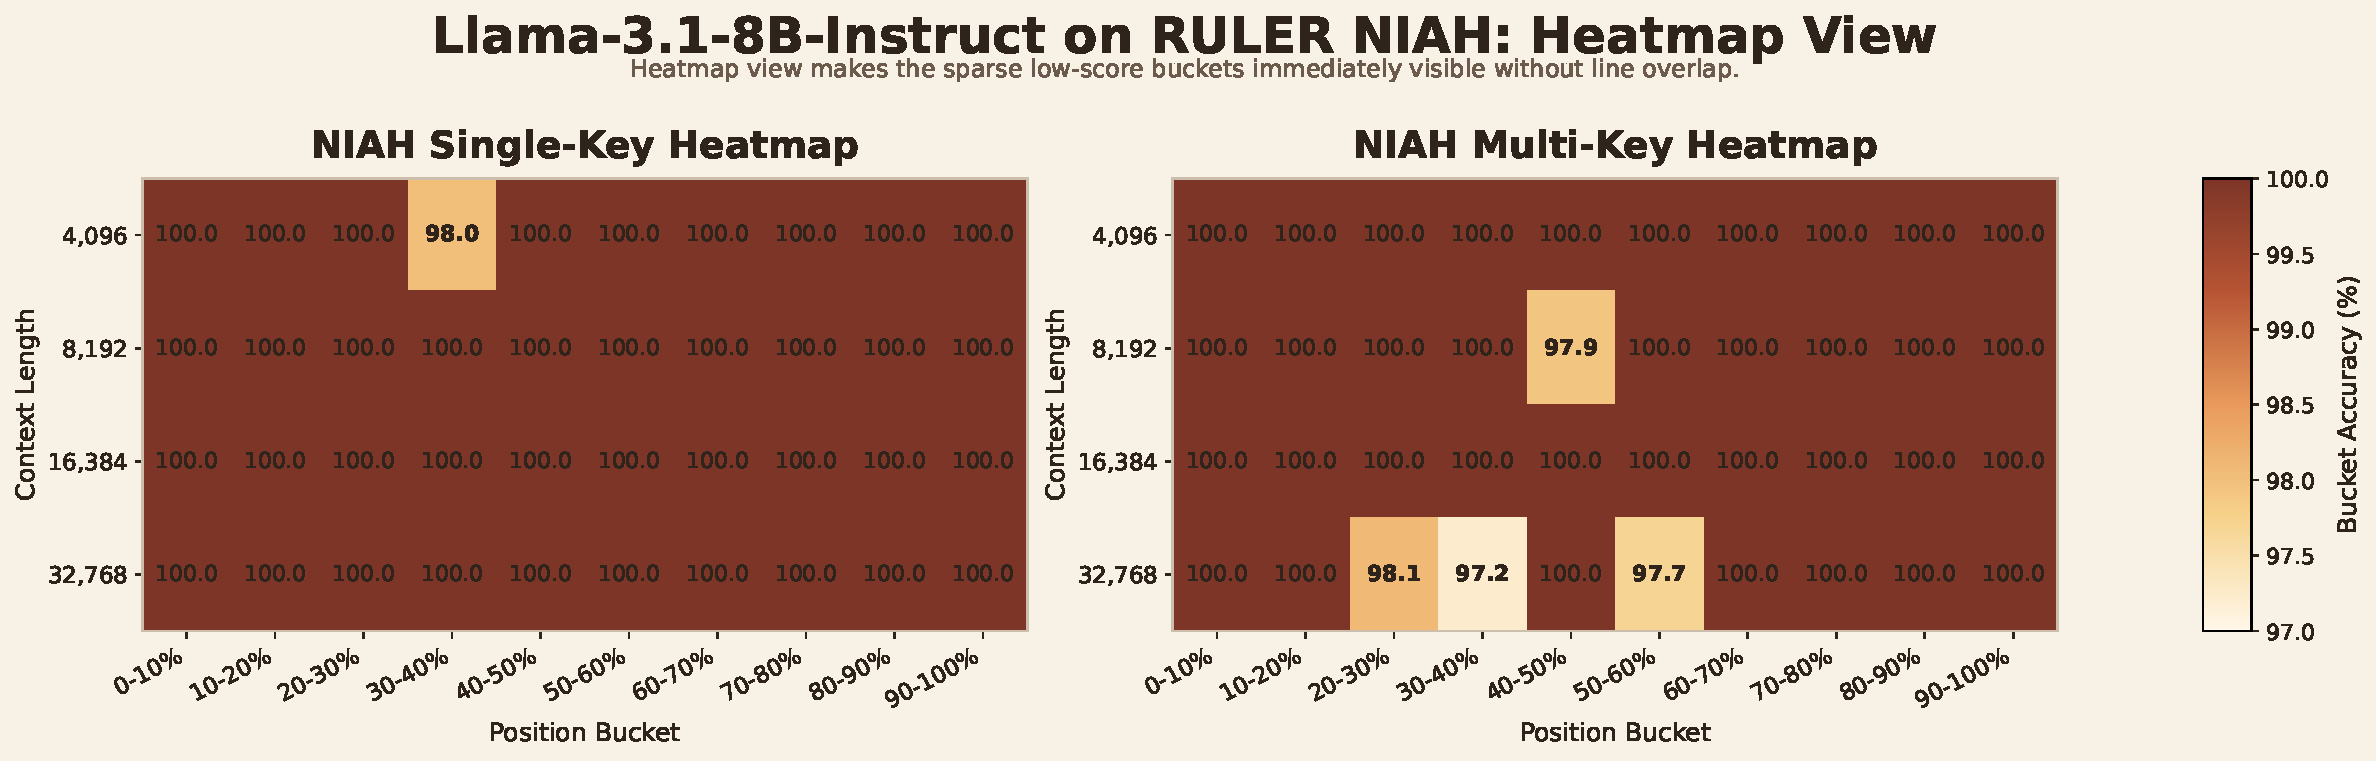
\includegraphics[width=0.78\textwidth]{../results/exp_a/llama31/position_sensitivity_llama31_heatmap.pdf}\\[0.8em]
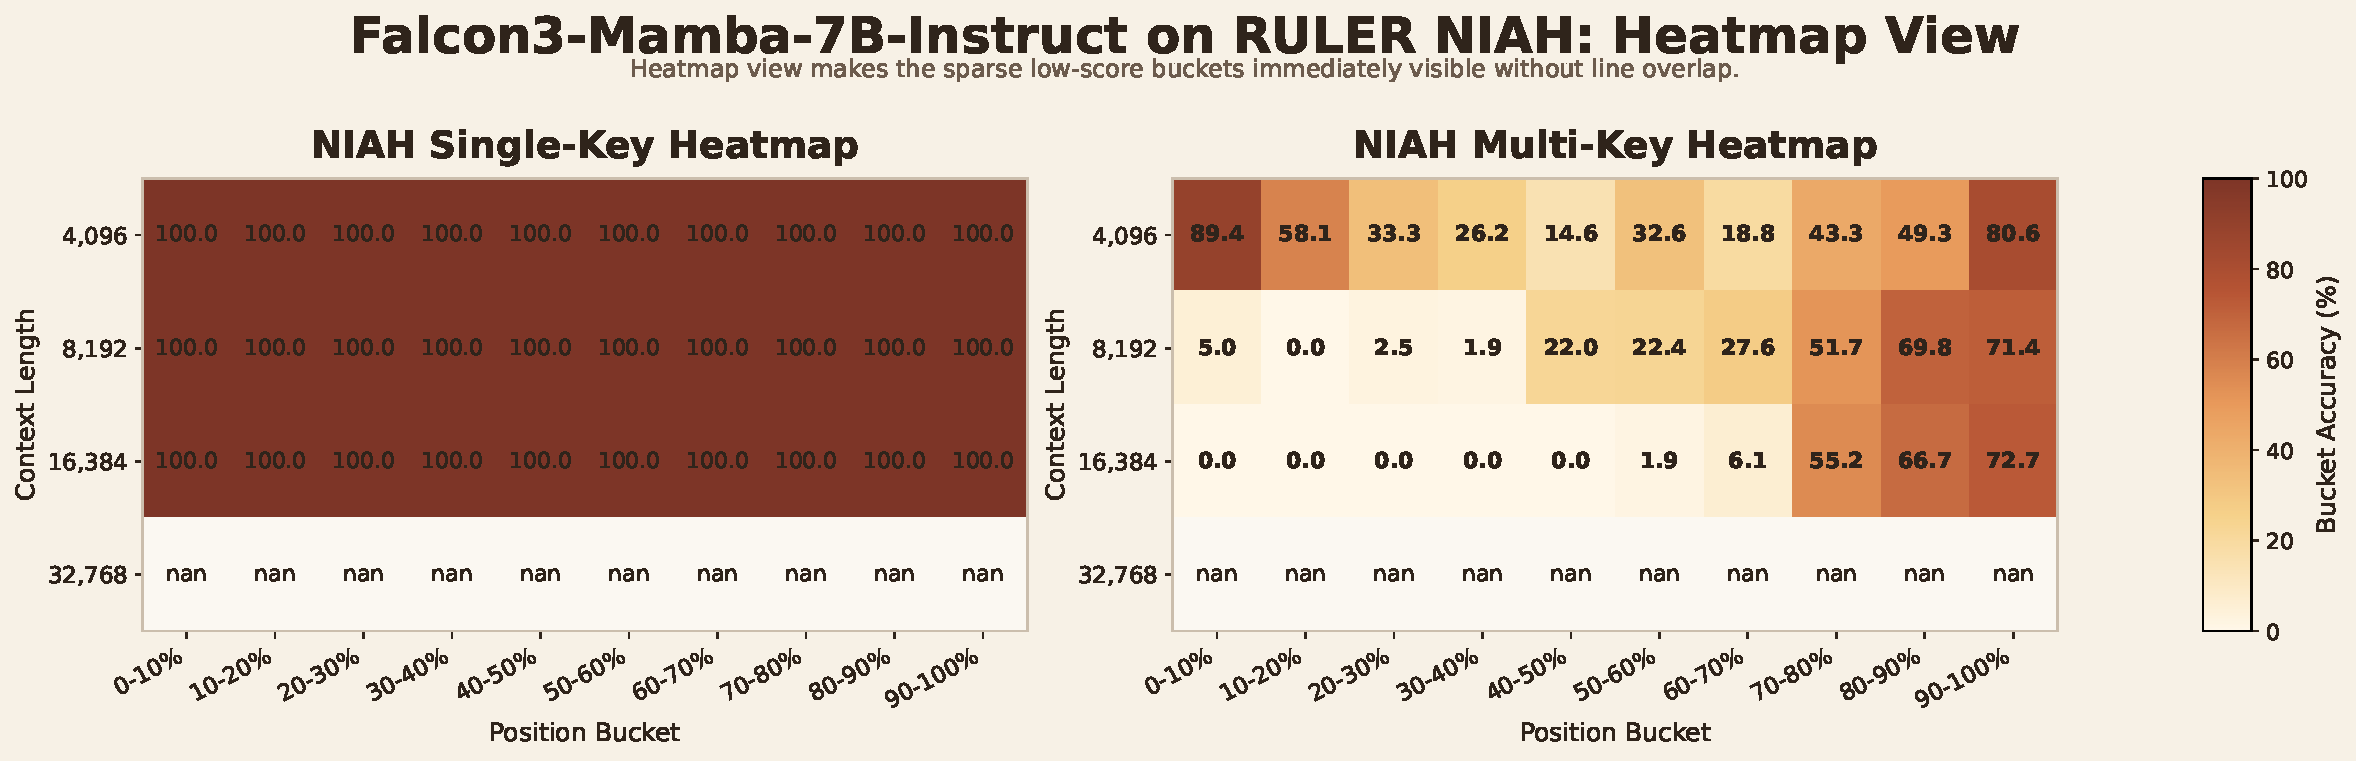
\includegraphics[width=0.78\textwidth]{../results/exp_a/mamba/position_sensitivity_mamba_heatmap.pdf}
\caption{Position-sensitive accuracy heatmaps. Top: Llama-3.1-8B-Instruct is near-saturated across lengths and positions. Bottom: Falcon3-Mamba-7B-Instruct is stable on single-key retrieval but degrades sharply on multi-key, especially in early-to-middle positions.}
\label{fig:expa-pos}
\end{figure}

\subsection{Experiment B1: Synthetic reasoning under context scaling}

We evaluate three RULER reasoning tasks: variable tracking (VT), common-word extraction (CWE), and frequent-word extraction (FWE). Unlike Exp~A, the goal is to measure whether reasoning degrades as a synthetic task is stretched to longer contexts while answer information remains available. For VT, we inject an answer-format suffix to encourage concise variable-name output (max 64 new tokens). CWE and FWE use the raw task prompts (max 120 and 50 tokens respectively). Each cell contains 500 examples.

Table~\ref{tab:expb-ruler} summarizes the results. For Llama, VT remains strong from 4K to 32K (99.8\% to 95.8\%), while CWE degrades sharply from 93.0\% at 4K to 0.6\% at 32K. FWE is non-monotonic, peaking at 86.0\% at 16K then dropping to 49.4\% at 32K. For Falcon3-Mamba, VT declines steadily from 55.0\% to 28.2\%, CWE is near floor at all lengths (0.2\% at 16K), and FWE is the best Mamba task but still degrades from 58.2\% to 44.4\%.

Figure~\ref{fig:expb-ruler-compare} visualizes the length-accuracy curves per task. Two points stand out. First, scores across VT, CWE, and FWE should not be interpreted as a ranking of intrinsic task difficulty, because the tasks differ in output format, answer set size, and decoding budget. The comparison is meaningful within each task across lengths and architectures. Second, the architectural contrast is consistent: Llama preserves stronger performance at longer lengths on all three tasks.

\begin{table}[t]
\centering
\caption{Exp B accuracy (\%) on RULER reasoning tasks.}
\label{tab:expb-ruler}
\begin{tabular}{lcccc}
\toprule
Model / Task & 4K & 8K & 16K & 32K \\
\midrule
Llama VT & 99.8 & 99.4 & 99.4 & 95.8 \\
Llama CWE & 93.0 & 81.2 & 41.4 & 0.6 \\
Llama FWE & 59.2 & 83.6 & 86.0 & 49.4 \\
Falcon3-Mamba VT & 55.0 & 40.2 & 28.2 & -- \\
Falcon3-Mamba CWE & 11.4 & 2.8 & 0.2 & -- \\
Falcon3-Mamba FWE & 58.2 & 63.8 & 44.4 & -- \\
\bottomrule
\end{tabular}
\end{table}

\begin{figure}[t]
\centering
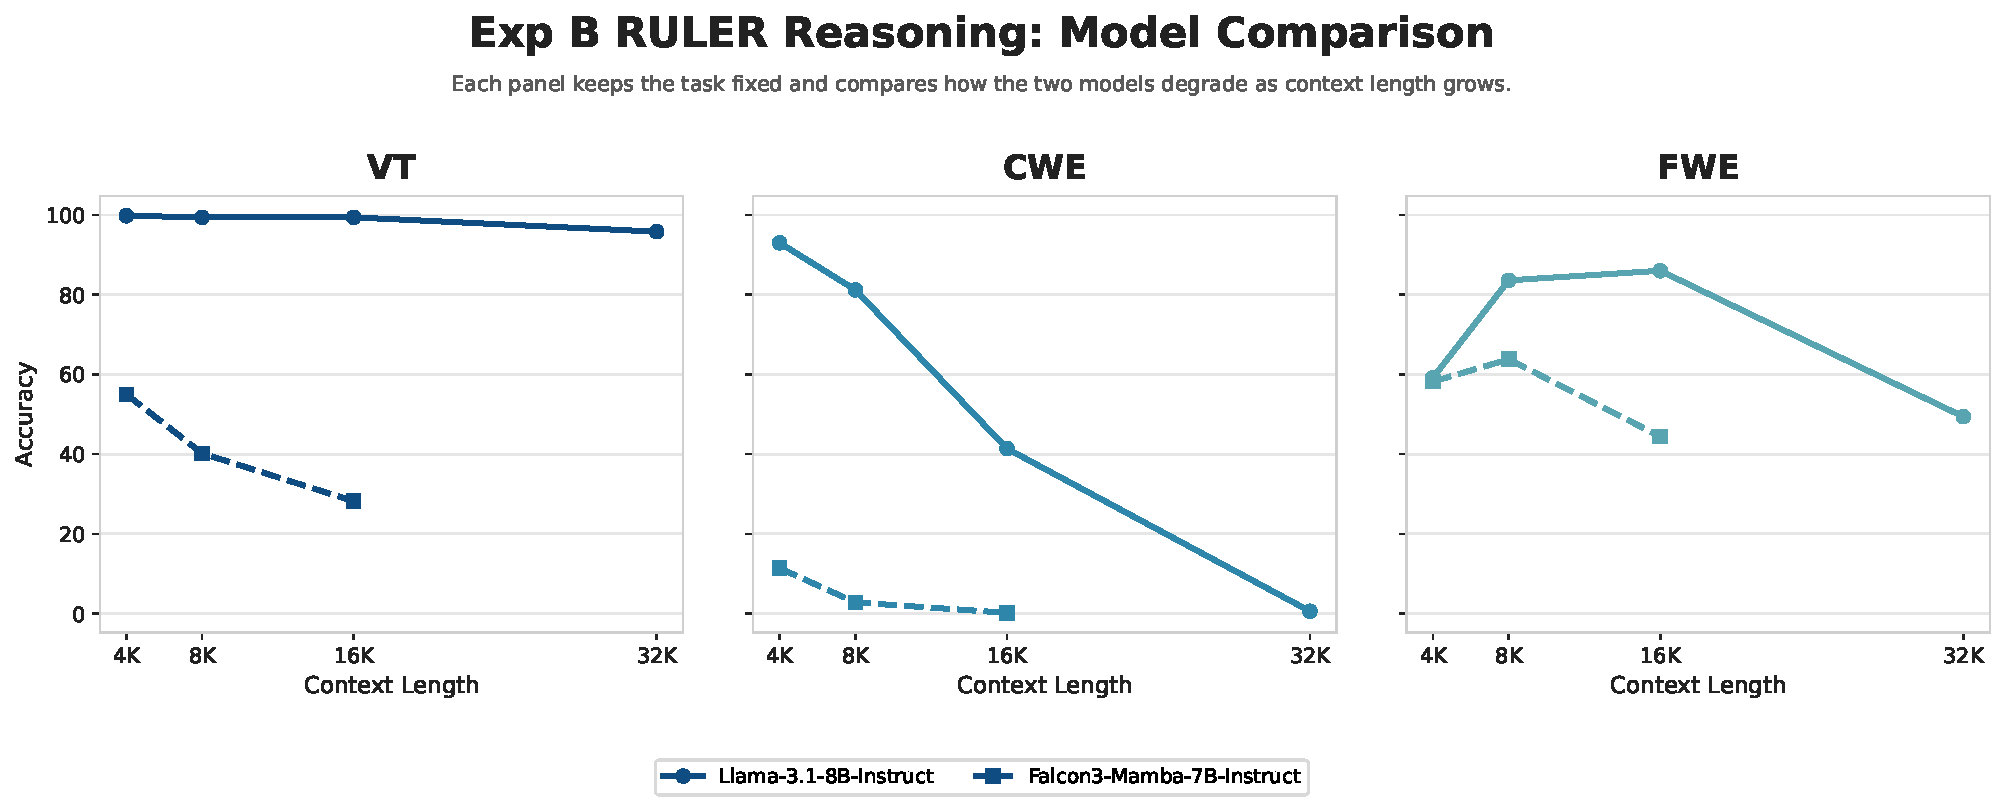
\includegraphics[width=0.97\textwidth]{../results/exp_b/ruler_reasoning/ruler_reasoning_model_compare.pdf}
\caption{Exp B RULER reasoning comparison curves. Each panel compares both models on one task as context length grows.}
\label{fig:expb-ruler-compare}
\end{figure}

\subsection{Experiment B2: Realistic tasks on LongBench}

We evaluate four LongBench tasks without artificial length bucketing: HotpotQA (multi-doc QA with multi-hop reasoning, QA-F1), Qasper (single-doc academic QA, QA-F1), GovReport (long-document summarization, Rouge-L F1), and RepoBench-P (code completion with repository context, edit similarity). Each task is run on its original samples. For Falcon3-Mamba, we apply a 20K-token input truncation budget to prevent OOM on the longest inputs.

Table~\ref{tab:expb-longbench} reports the results. Llama outperforms Mamba on all four tasks. The gap is largest on HotpotQA (51.09 vs.\ 29.38 QA-F1), consistent with the multi-hop nature of the task. Both models struggle on GovReport and RepoBench-P, where even the better model reaches only 17.50 Rouge-L F1 and 9.95 edit similarity. These absolute scores indicate that real-world long-context tasks remain challenging for both architectures, with the Transformer retaining a clear advantage.

\begin{table}[t]
\centering
\caption{Exp B LongBench results. All metrics are task-specific (QA-F1 for HotpotQA/Qasper, Rouge-L F1 for GovReport, edit similarity for RepoBench-P).}
\label{tab:expb-longbench}
\begin{tabular}{lccc}
\toprule
Task (Metric) & Llama-3.1-8B & Falcon3-Mamba-7B \\
\midrule
HotpotQA (QA-F1) & 51.09 & 29.38 \\
Qasper (QA-F1) & 26.34 & 22.48 \\
GovReport (Rouge-L) & 17.50 & 14.58 \\
RepoBench-P (Edit Sim) & 9.95 & 8.71 \\
\bottomrule
\end{tabular}
\end{table}

\subsection{Experiment C: System serving performance}

We benchmark system efficiency using a synthetic fill text with fixed 128-token output generation. Three configurations are tested: Llama-3.1 on vLLM \citep{kwon2023pagedattention}, Llama-3.1 on HuggingFace Transformers, and Falcon3-Mamba on HuggingFace Transformers. Context lengths range from 4K to 32K; batch sizes include 1, 4, 8, and 16 (vLLM only). Metrics measured are TTFT, TPOT, throughput (tokens/s), and peak GPU memory.

\paragraph{Prefill latency.}
Figure~\ref{fig:expc-ttft} shows TTFT as a function of context length. For vLLM at batch size 1, TTFT grows from 380\,ms at 4K to 4331\,ms at 32K---roughly $\mathcal{O}(L^2)$ scaling. At batch size 16, the 32K TTFT reaches 57.9\,s, making interactive use infeasible. HuggingFace TTFT is comparable to vLLM at batch size 1 for the same model. Mamba HF shows similar prefill scaling (2257\,ms at 16K), consistent with its Transformer-like prefill stage despite recurrent decoding.

\begin{figure}[t]
\centering
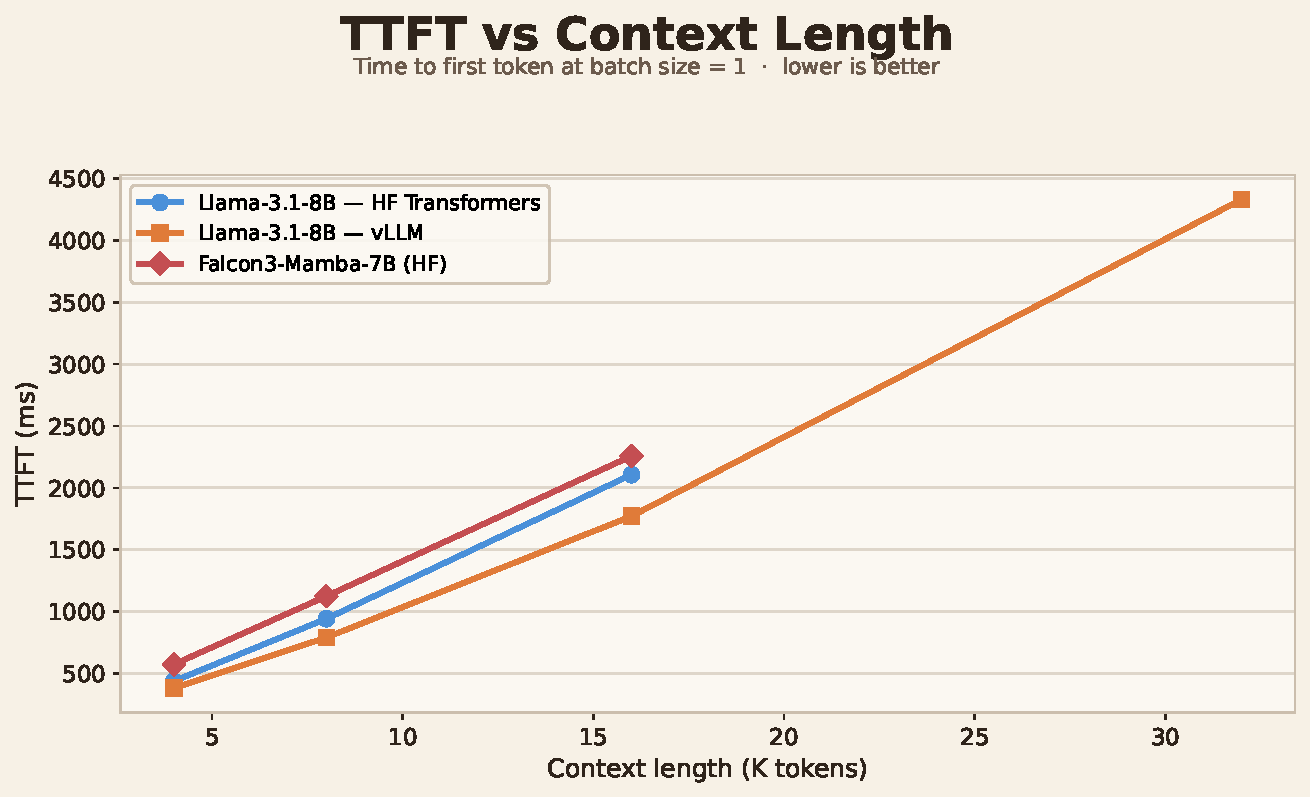
\includegraphics[width=0.85\textwidth]{../results/exp_c/fig1_ttft_vs_context.pdf}
\caption{TTFT vs.\ context length. vLLM shown at batch sizes 1 and 16; HF backends at batch size 1. Prefill cost dominates at long contexts.}
\label{fig:expc-ttft}
\end{figure}

\paragraph{Decode efficiency.}
Mamba's TPOT is nearly constant at 73--74\,ms/token across all context lengths, reflecting the $\mathcal{O}(1)$ per-step cost of state-space recurrence. Llama's TPOT grows from 19 to 22\,ms/token (vLLM) and from 28 to 46\,ms/token (HF) as context increases, consistent with $\mathcal{O}(L)$ decode cost from growing KV-cache access.

\paragraph{Throughput and batching.}
Figure~\ref{fig:expc-throughput} shows throughput vs.\ batch size. At 4K, vLLM throughput scales from 46 to 176\,tok/s as batch size grows from 1 to 16. At 32K, throughput saturates at approximately 18\,tok/s regardless of batch size, because prefill dominates the end-to-end time. HF throughput is consistently lower: 32\,tok/s at 4K/bs1 vs.\ 46\,tok/s for vLLM.

\begin{figure}[t]
\centering
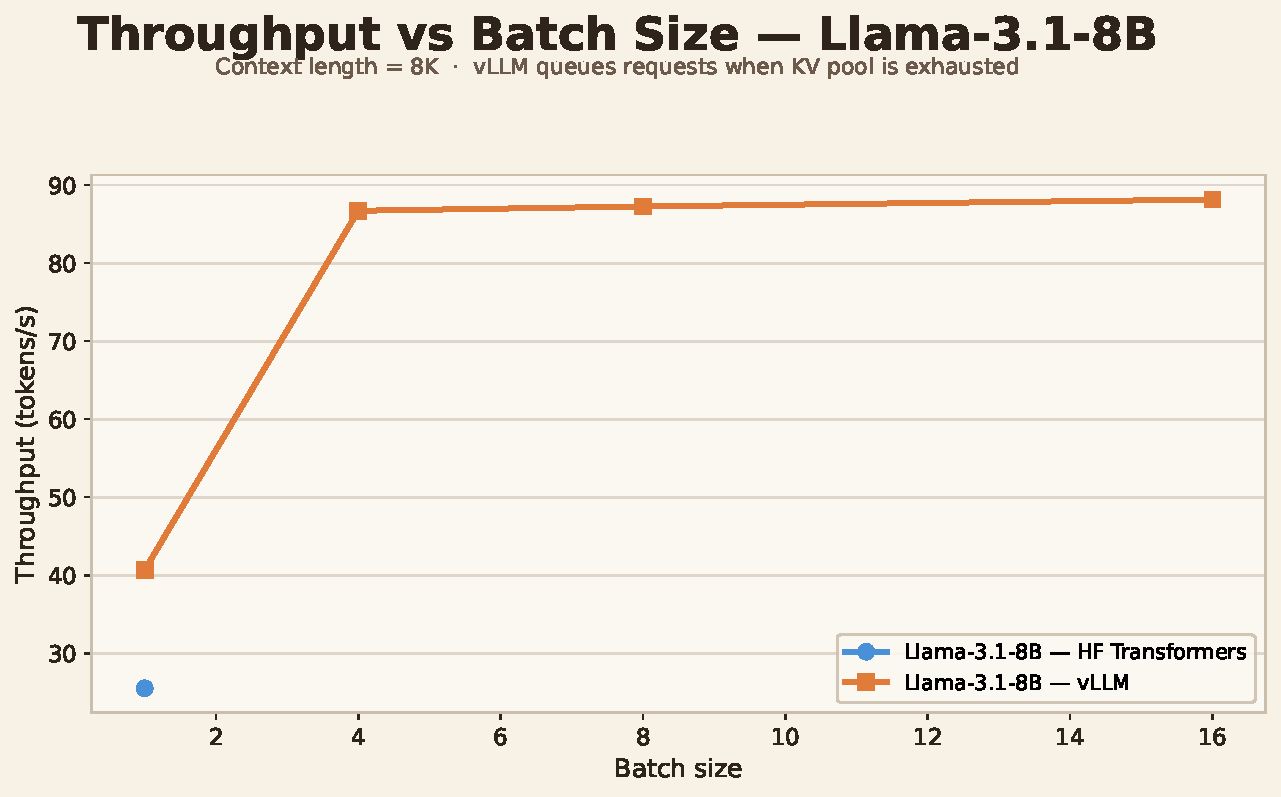
\includegraphics[width=0.85\textwidth]{../results/exp_c/fig3_throughput_vs_batch.pdf}
\caption{Throughput vs.\ batch size. vLLM benefits from batching at shorter contexts but saturates under prefill dominance at 32K.}
\label{fig:expc-throughput}
\end{figure}

\paragraph{Memory.}
Figure~\ref{fig:expc-memory} shows peak GPU memory. vLLM memory is flat at 21.77\,GB across all configurations (model weights dominate). HF memory grows from 17.1\,GB (4K) to 20.2\,GB (16K) for Llama, and from 16.4\,GB (4K) to 21.8\,GB (16K) for Mamba. Memory is the binding constraint for 32K Mamba: the 24\,GB GPU cannot accommodate the combined model and KV-cache footprint.

\begin{figure}[t]
\centering
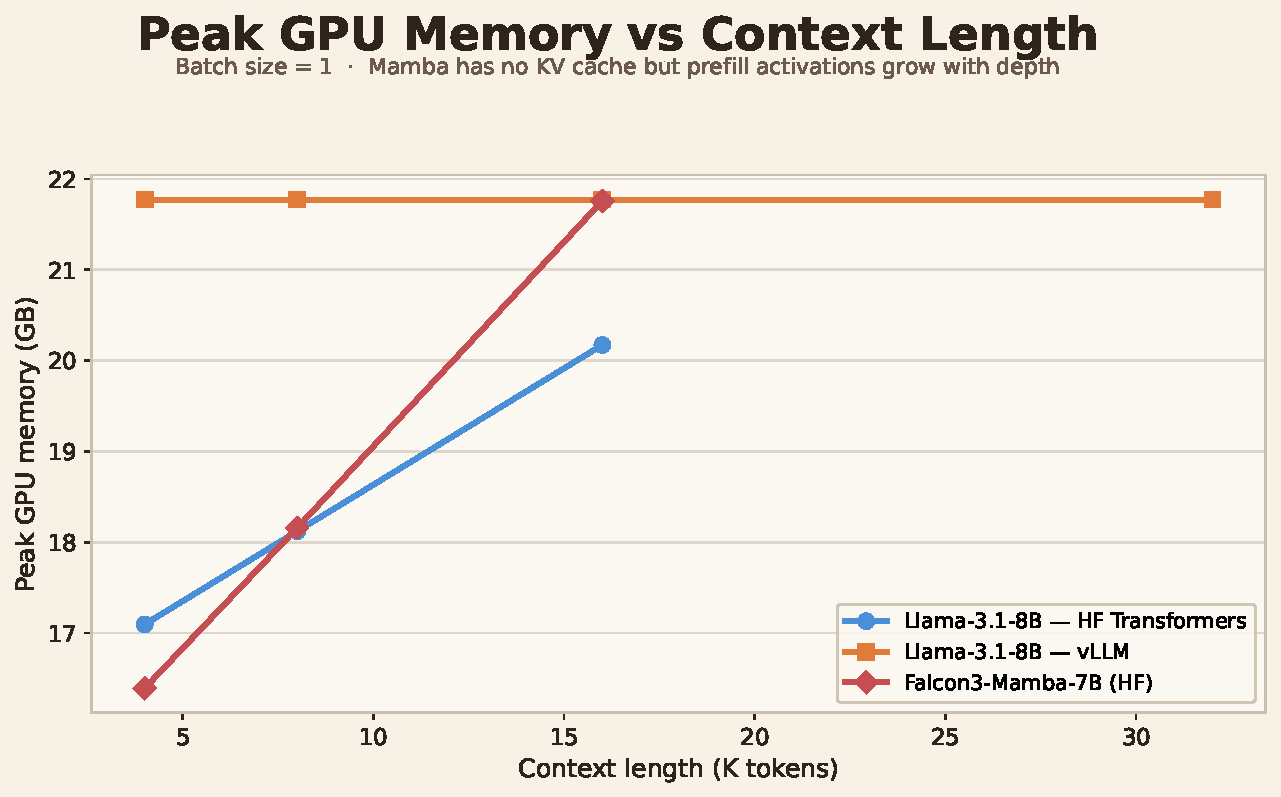
\includegraphics[width=0.85\textwidth]{../results/exp_c/fig2_memory_vs_context.pdf}
\caption{Peak GPU memory vs.\ context length. vLLM memory is dominated by model weights; HF memory grows with context due to KV-cache.}
\label{fig:expc-memory}
\end{figure}

\paragraph{Implications.}
The system results confirm that prefill cost and memory, not decode speed, are the primary barriers to long-context serving under realistic batch workloads. The flat Mamba TPOT demonstrates the theoretical advantage of $\mathcal{O}(1)$ per-step decoding, but this advantage is offset by higher absolute decode cost and memory constraints that prevent Mamba from reaching 32K on commodity hardware.

\subsection{Summary of experimental findings}
Three patterns emerge across experiments. First, retrieval failure is task-dependent: single-key success does not imply multi-key robustness, and the gap widens with context length. Second, reasoning under context scaling reveals heterogeneous degradation: within the same model, variable tracking is much more stable than common-word extraction, suggesting that the reasoning operation itself---not just context length---determines stability. Third, system constraints interact with model architecture to define usable context: Mamba's stable TPOT is compromised by memory limits that prevent 32K evaluation, while Llama's strong retrieval and reasoning are available at 32K but with rapidly growing prefill cost. These patterns jointly support the central thesis: long-context ability is not a scalar but a joint function of architecture, task, and infrastructure.

\section{Discussion}
\label{sec:discussion}

\subsection{Long-context ability is not a single dimension}
The experiments confirm what the survey suggests: neither retrieval, reasoning, nor serving efficiency alone captures long-context ability. Falcon3-Mamba is perfect on single-key retrieval yet fails dramatically on multi-key binding. Llama maintains strong variable tracking through 32K while common-word extraction collapses to near-zero. This task-dependent degradation pattern is consistent across both architectures, reinforcing that ``long-context'' is an umbrella term for distinct capabilities that can fail independently.

\subsection{Nominal vs.\ effective context}
The gap between nominal and effective context is large and task-dependent. Llama's nominal 128K window maps to near-perfect retrieval effectiveness at 32K, but CWE reasoning effectiveness drops below 50\% by 16K. Mamba's nominal 32K is cut to 16K by memory constraints before task performance is even considered. This suggests that $L_{\mathrm{eff}}$ should be reported per task family rather than as a single number, and that system feasibility should be a first-class constraint on claimed capability.

\subsection{Architecture matters, but not uniformly}
The Transformer retains a clear advantage on retrieval under interference and on reasoning stability across our tested range. The state-space model's advantage is not in accuracy but in decode efficiency: Mamba's constant per-step cost is genuine and measurable. However, this efficiency is offset by weaker content-addressable retrieval and larger absolute per-token latency. The practical conclusion is comparative: different architectures fail differently, and the failure mode matters for downstream use.

\subsection{System constraints as first-class factors}
Exp~C demonstrates that prefill cost and memory, not model quality, are the limiting factors for long-context deployment. vLLM throughput saturates at 18\,tok/s at 32K regardless of batch size, and 32K Mamba is not reachable on a 24\,GB GPU. These are not mere engineering details; they define which context lengths are usable. The serving dimension should be evaluated alongside retrieval and reasoning, not as an afterthought.

\subsection{Limitations}
Our study has several limitations. The model set is small (two architectures) and the hardware is restricted to a single 24\,GB GPU. The prompt policy is task-dependent: VT uses an answer-format suffix that may inflate scores relative to CWE and FWE, limiting cross-task score comparison. LongBench tasks are not length-bucketed, which prevents straightforward length-degradation analysis. The system benchmark uses synthetic fill text rather than real prompts, which may understate KV-cache access patterns. The Mamba 32K gap is a hardware constraint, not an architectural claim; on larger GPUs, 32K may be reachable and should be evaluated.

\section{Conclusion}
\label{sec:conclusion}

This report surveyed long-context LLMs through five dimensions---nominal context length, effective retrieval, long-range reasoning, inference-time extension, and system serving efficiency---and presented experimental evidence across retrieval, reasoning, and system benchmarks. The survey shows that no single technical route fully determines long-context ability. The experiments confirm that architecture, task structure, and system constraints jointly determine usable context.

The empirical findings are consistent with the survey's main thesis. Retrieval is not monolithic: single-key success does not transfer to multi-key robustness. Reasoning degrades heterogeneously: some operations remain stable at 32K while others collapse at 16K. System constraints define the boundary of what is empirically testable: prefill latency makes 32K serving slow even with optimized engines, and GPU memory excludes 32K for state-space models on commodity hardware.

The practical message is that long-context evaluation, model comparison, and system design should all account for this multi-dimensional nature. Reporting a single context length or a single benchmark score is insufficient. Effective context should be reported per task family, and serving feasibility should be treated as a first-class evaluation criterion alongside accuracy.

\bibliographystyle{plainnat}
\bibliography{references}

\end{document}
